\documentclass{beamer}
\usetheme{metropolis} % Use metropolis theme
\usepackage[utf8]{inputenc}
%\usepackage[portuguese]{babel}
\usepackage{lipsum}
\usepackage{ragged2e}
\usepackage{etoolbox}
\usepackage{graphicx}

\title{Simulador de processos}
\date{\today}
\author{Gabriel Capella - 8962078 e Luís Felipe de Melo - 9297961}
\institute{Centre for Modern Beamer Themes}
\begin{document}
\maketitle

\section{Considerações sobre o escalonador}
\begin{frame}{Princípios}
	\begin{itemize}
		\item Um processo só pode ser criado a partir de outro.
		\item O escalonador deve ter um processo em sua fila antes de iniciar.
		\item Se não há nenhum processo a ser executado, desligamos todos as CPUs.
	\end{itemize}
\end{frame}


\begin{frame}{Como implementamos}
	Os três tipos de escalonadores devem apresentar as seguintes funções:
	\begin{itemize}
		\item \textsc{p\_init}: função chamada para ligar o nosso escalonador. Ela verifica quantas CPUs há no computador do usuário e inicia uma thread para cada uma. Finaliza somente quando não há mais processos a serem executados.
		\item \textsc{p\_exec}: recebe as características de um novo processo (nome, linha do trace, tempo de execução, ponteiro para função e argumentos da função). Adiciona esse processo ao escalonador.
		\item \textsc{p\_run}: chamada dentro de um processo, verifica se ele deve continuar sua execução ou parar.
	\end{itemize}
\end{frame}


\begin{frame}{Processo \textsc{load\_process} (-1)}
	\justifying
	Antes do nosso escalonador iniciar, adicionamos esse processo a ele. Esse processo tem a função criar os nossos outros processos. Ou seja, ele verifica se já está na hora de adicionar outros processos no escalonador baseado no arquivo de trace. 
	
	Quando existem processos pedentes a serem criados, ele espera 0,05s e depois adiciona a si mesmo no escalonador. 
\end{frame}


\begin{frame}{Exemplo}
	Vamos executar esse exemplo com os 4 algoritmos e pintar cada processo com uma cor.
	\begin{columns}[T,onlytextwidth]
		\column{0.5\textwidth}
		
		0 1 processo1 20 \newline
		0 2 processo2 20 \newline
		0 3 processo3 20 \newline
		0 4 processo4 20 \newline
		1 5 processo1 20 \newline
		1 6 processo2 20 \newline
		1 7 processo3 20 \newline
		1 8 processo4 20 \newline
		
		\column{0.5\textwidth}
		
		\metroset{block=fill}
		
		
		1.5 processo9 1 20 \newline
		1.5 processo10 2 20 \newline
		1.5 processo11 3 20 \newline
		1.5 processo12 4 20 \newline
		5 13 processo1 20 \newline
		5 14 processo2 20 \newline
		5 15 processo3 20 \newline
		5 16 processo4 20
		
		
	\end{columns}
\end{frame}

\begin{frame}{Exemplo}
	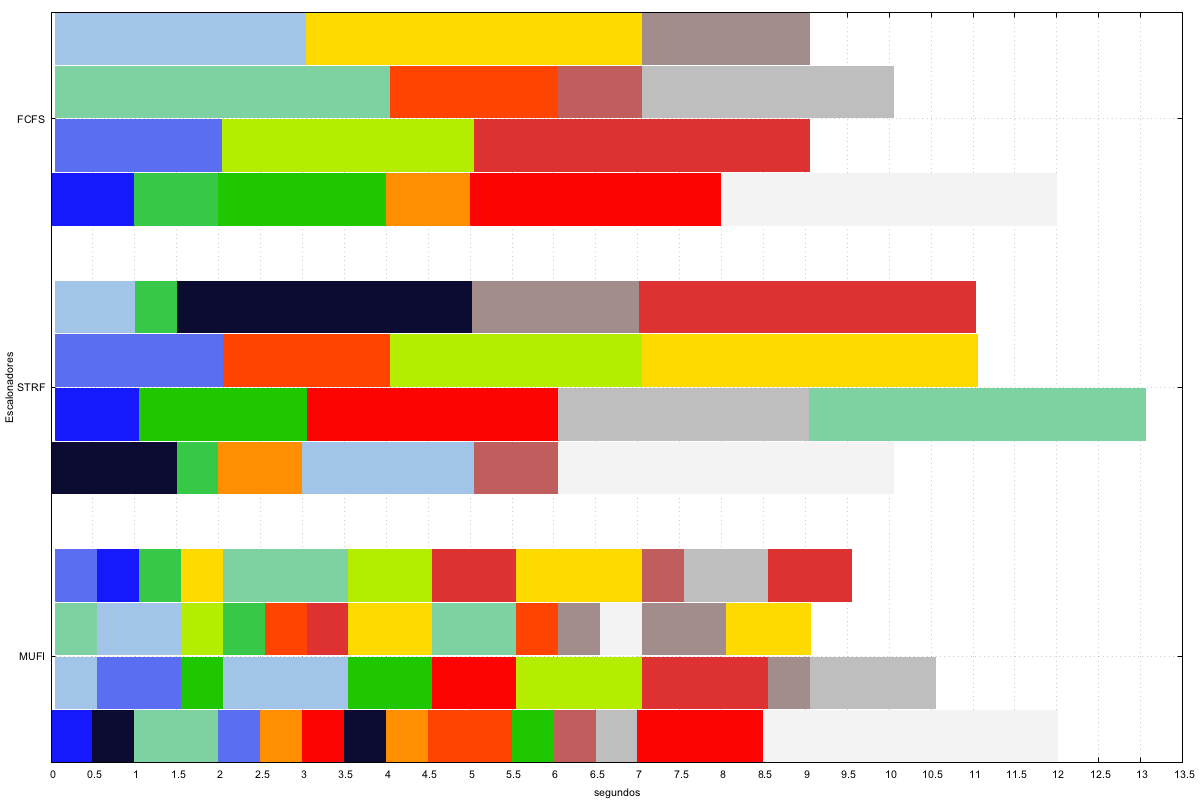
\includegraphics[width=\textwidth]{graphs/comparacao}
	
	{\tiny *Nesse exemplo o load\_process está com intervalos de 0,5s.}
\end{frame}

\section{Testes}

\begin{frame}{Gerando valores}
	\justifying
	Escolhemos um número de processos $n$ e escolhemos um valor $x$ entre  0 e 10, uniformemente. Depois escolhemos $y$ entre $x$ e 10. $x$ é o momento em que o processo inicia e $y-x$ é a duração do processo. Considere as unidades em segundos.
	
	Veja que $\overline{x} = 5.0$ e $\overline{y} = 7.5$ e portanto o tempo médio dos nossos processos é de 2.5s.
\end{frame}


\begin{frame}{Tempo Gasto}
	\begin{columns}[T,onlytextwidth]
		\column{0.5\textwidth}
		\justifying
		Utilizamos $n = 10, 100, 500$ e realizamos 30 testes para cada tipo de escalonador para 4 e 8 processadores. Sabendo que o tempo médio esperado era 2.5s, o tempo total gasto previsto foi de $610 \times 30 \times 3 \times 2.5s \times 2 = 274500s$, que equivale a $76.25h$.
		
		Para agilizar o processo utilizamos um serviço de cloud com a seguinte configuração descrita ao lado.
		
		\column{0.5\textwidth}
		
		\metroset{block=fill}
		\begin{center}
			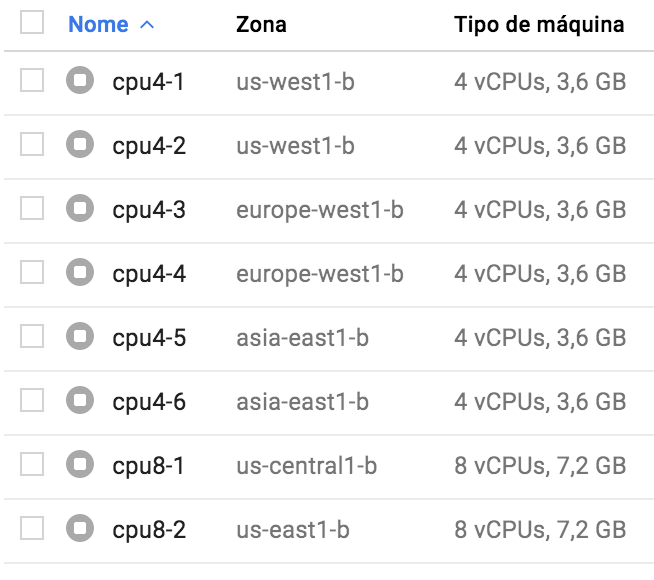
\includegraphics[scale=0.4]{cloud}
		\end{center}
		
	\end{columns}
	
	
	{\tiny *Finalizamos tudo em menos de 3h! 38.125h de processamento em duas máquinas de 8 núcleos, resulta em aproximadamente 2.4h.}
\end{frame}


\begin{frame}{Trocas de Contexto, $n = 10$ e $4$ CPUs}
	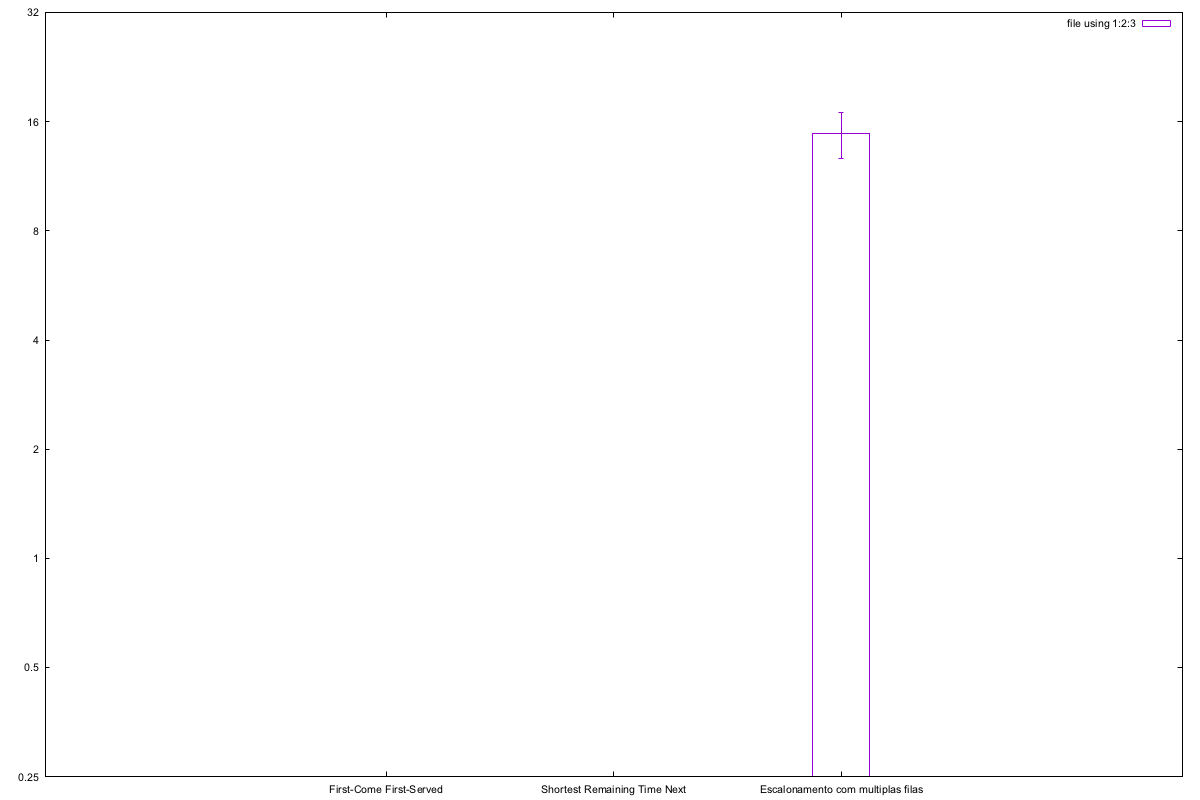
\includegraphics[width=\textwidth]{graphs/testes_capella/result/trocas-r4-10}
\end{frame}


\begin{frame}{Trocas de Contexto, $n = 10$ e $8$ CPUs}
	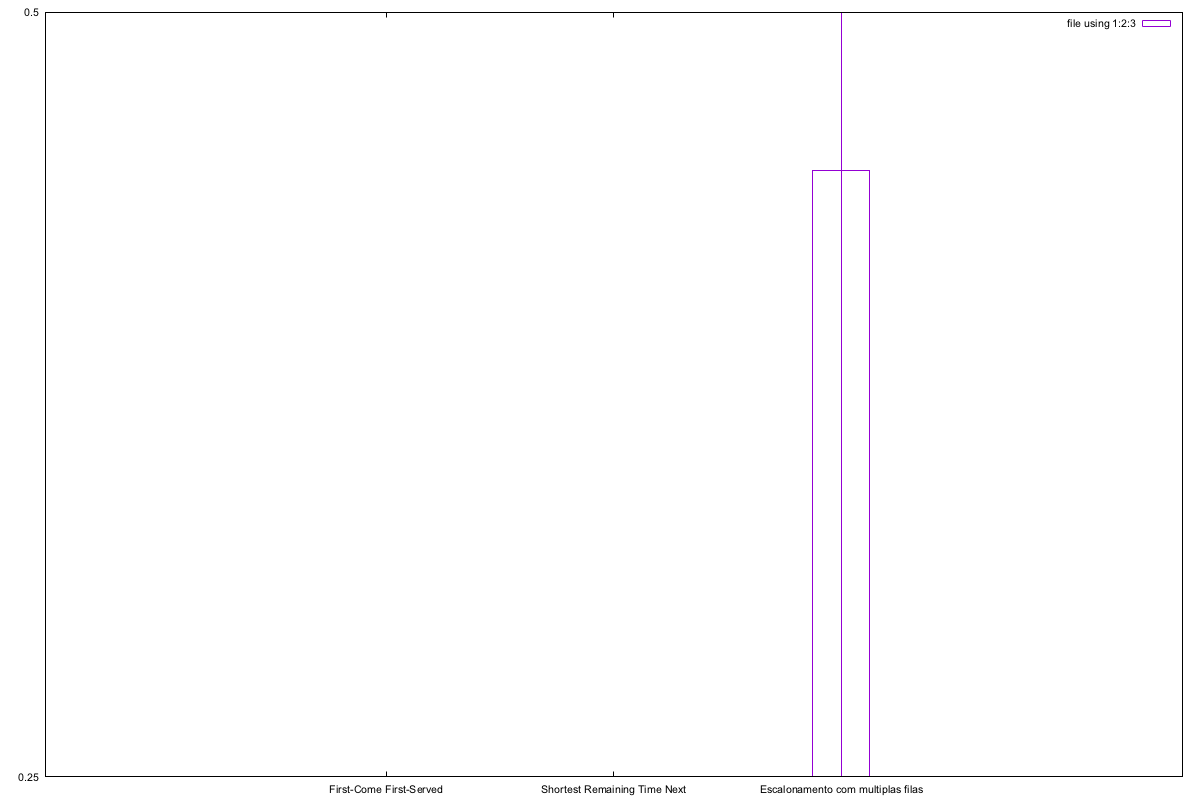
\includegraphics[width=\textwidth]{graphs/testes_capella/result/trocas-r8-10}
\end{frame}


\begin{frame}{Trocas de Contexto, $n = 100$ e $4$ CPUs}
	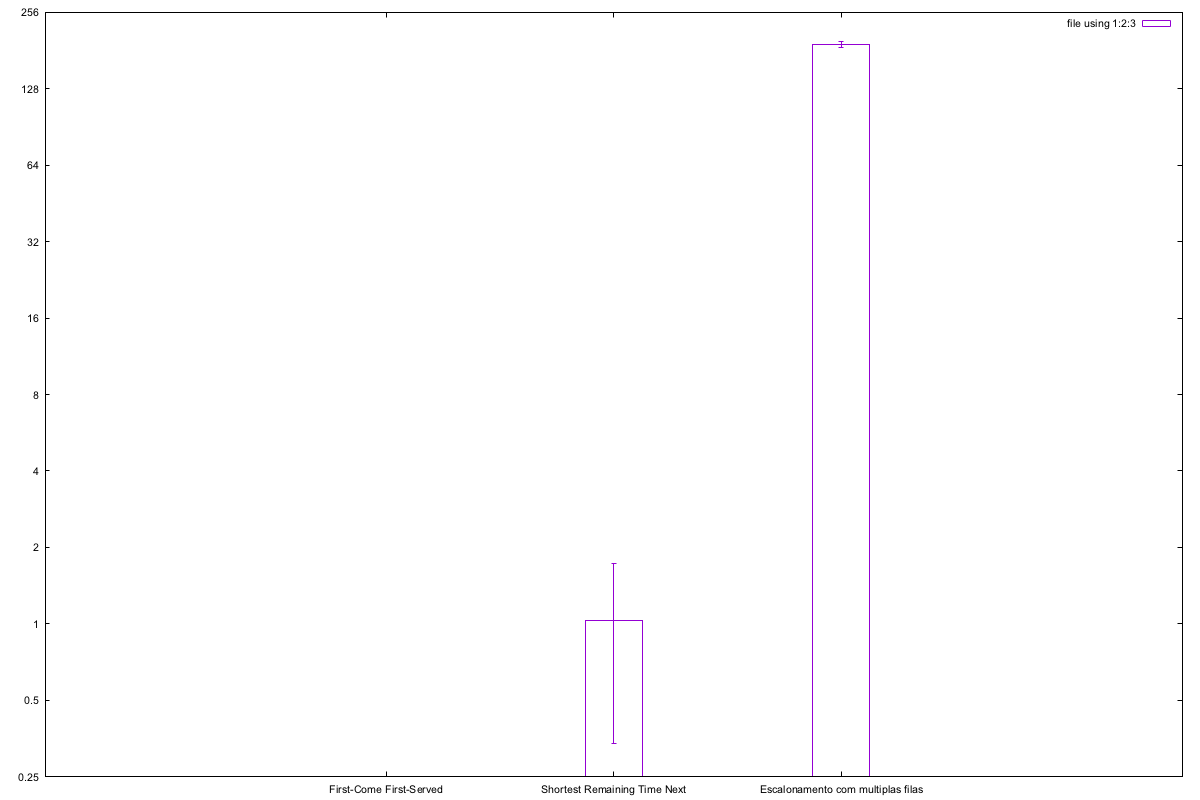
\includegraphics[width=\textwidth]{graphs/testes_capella/result/trocas-r4-100}
\end{frame}


\begin{frame}{Trocas de Contexto, $n = 100$ e $8$ CPUs}
	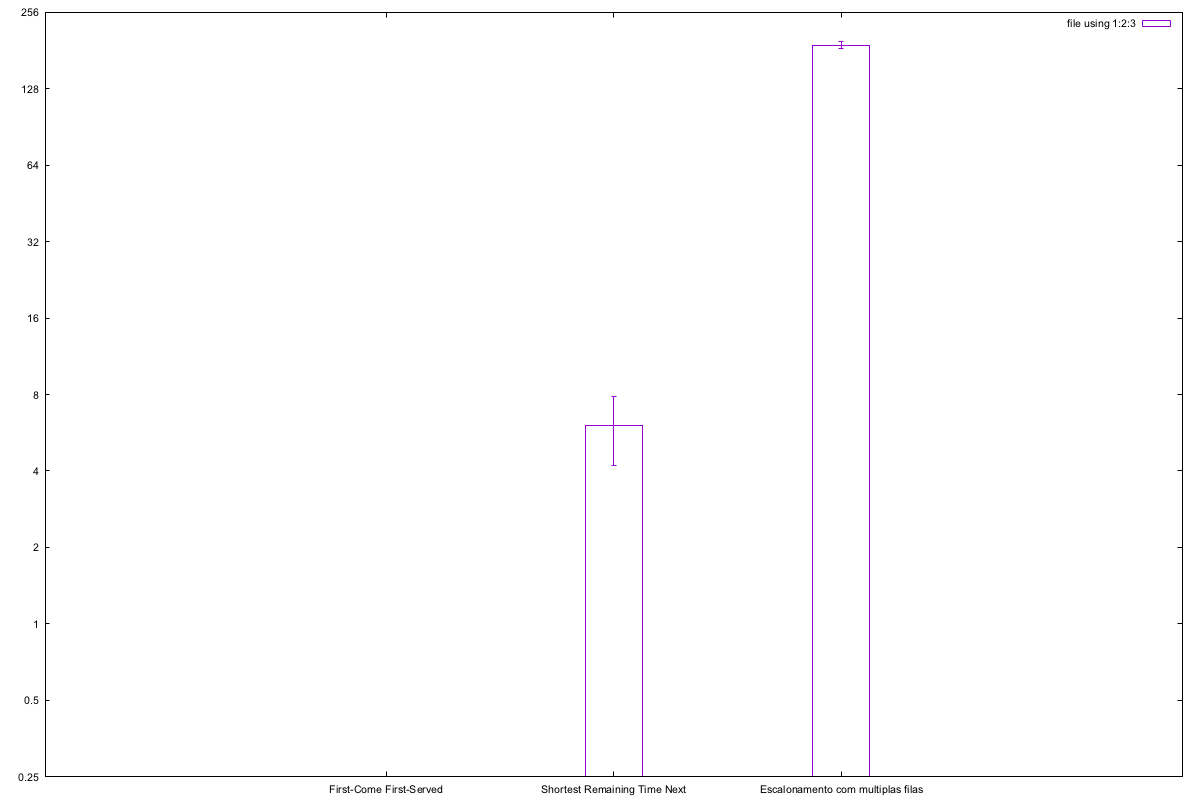
\includegraphics[width=\textwidth]{graphs/testes_capella/result/trocas-r8-100}
\end{frame}


\begin{frame}{Trocas de Contexto, $n = 500$ e $4$ CPUs}
	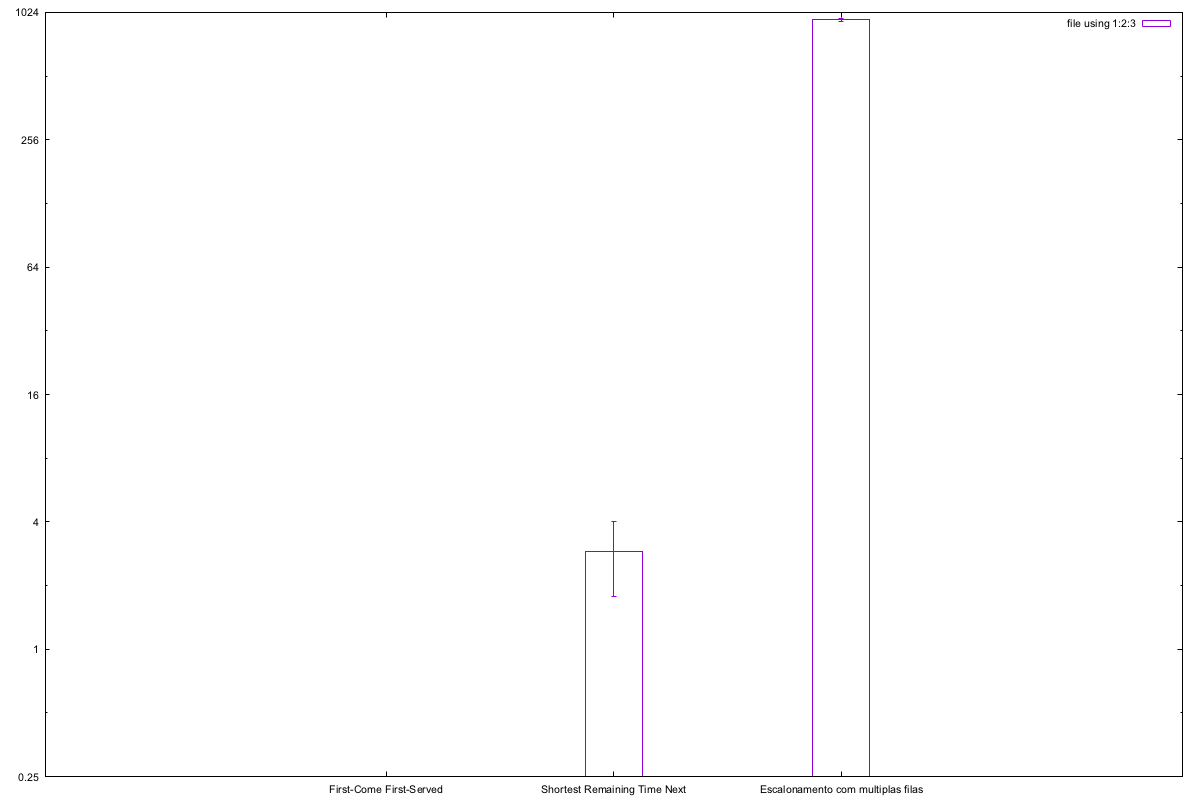
\includegraphics[width=\textwidth]{graphs/testes_capella/result/trocas-r4-500}
\end{frame}


\begin{frame}{Trocas de Contexto, $n = 500$ e $8$ CPUs}
	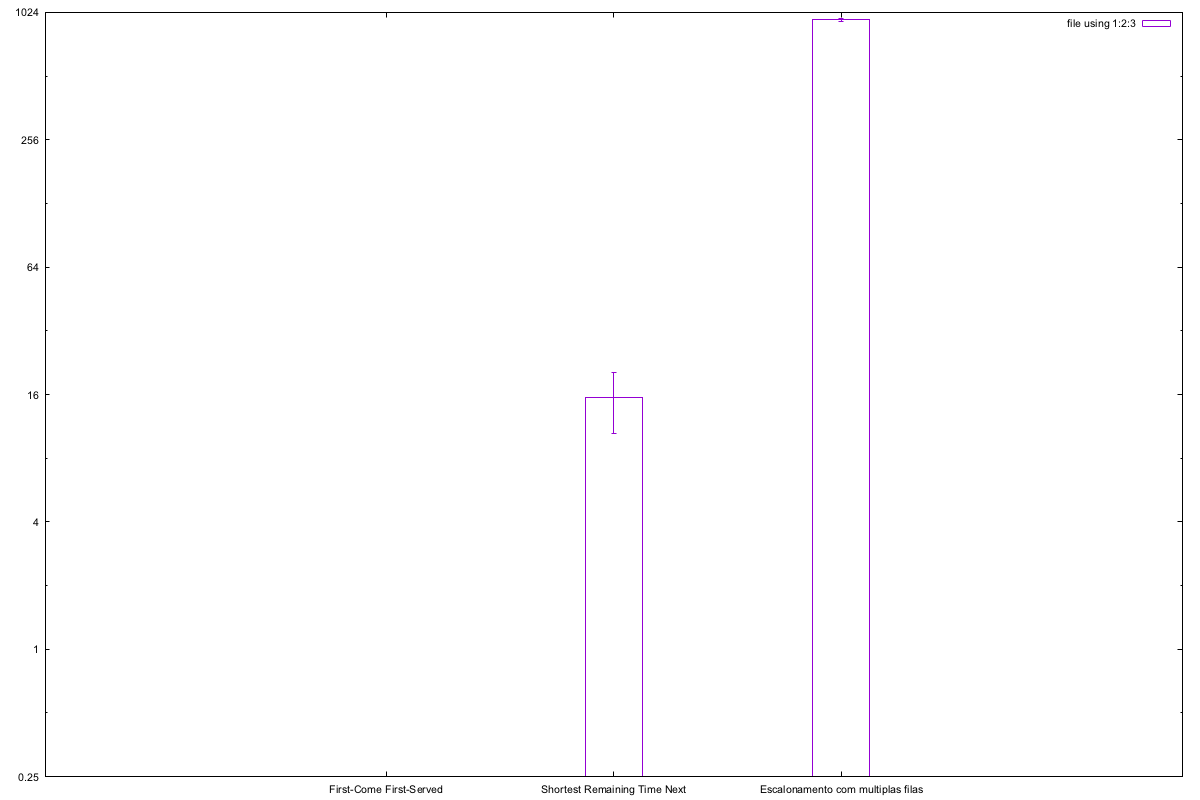
\includegraphics[width=\textwidth]{graphs/testes_capella/result/trocas-r8-500}
\end{frame}

\begin{frame}{Porcentagem de Deadlines Cumpridos, $n = 10$ e $4$ CPUs}
	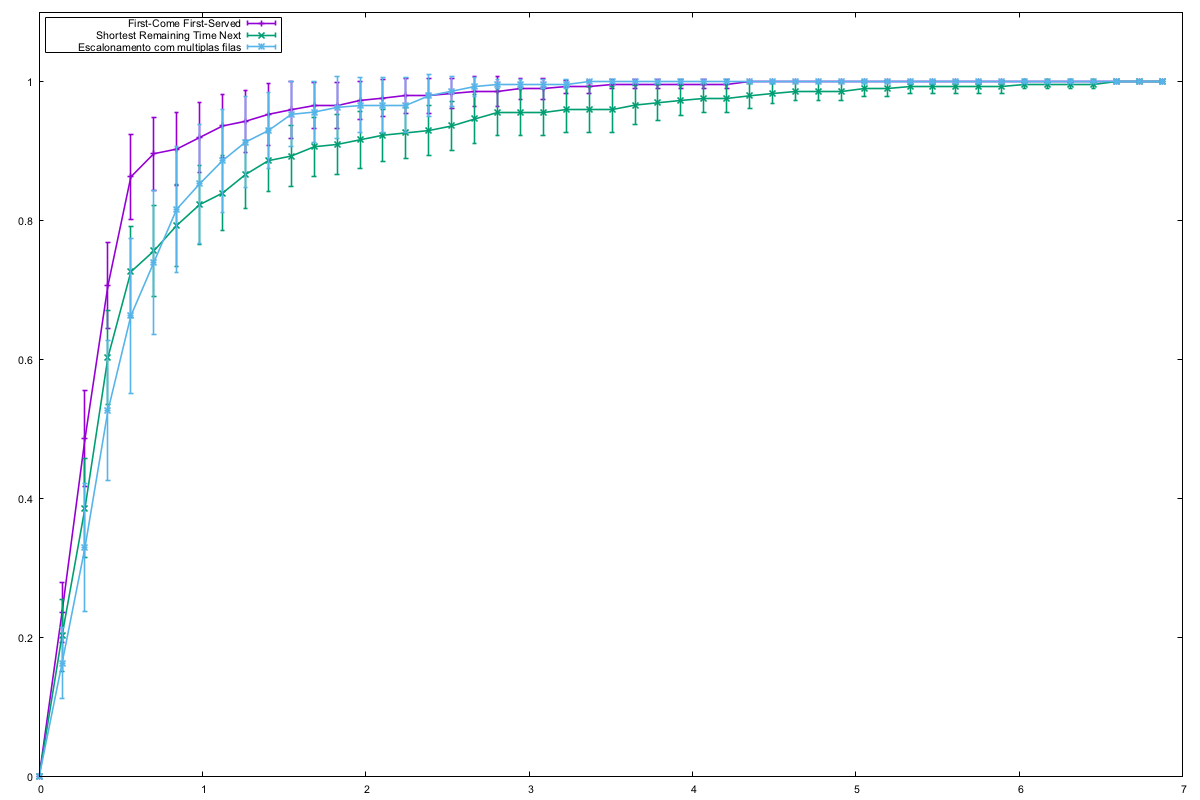
\includegraphics[width=\textwidth]{graphs/testes_capella/result/deadlines-r4-10}
	
	{\tiny No eixo $x$ temos o tempo em segundos que foi adicionado $y$ do processo para determinar o deadline.}
\end{frame}


\begin{frame}{Porcentagem de Deadlines Cumpridos, $n = 10$ e $8$ CPUs}
	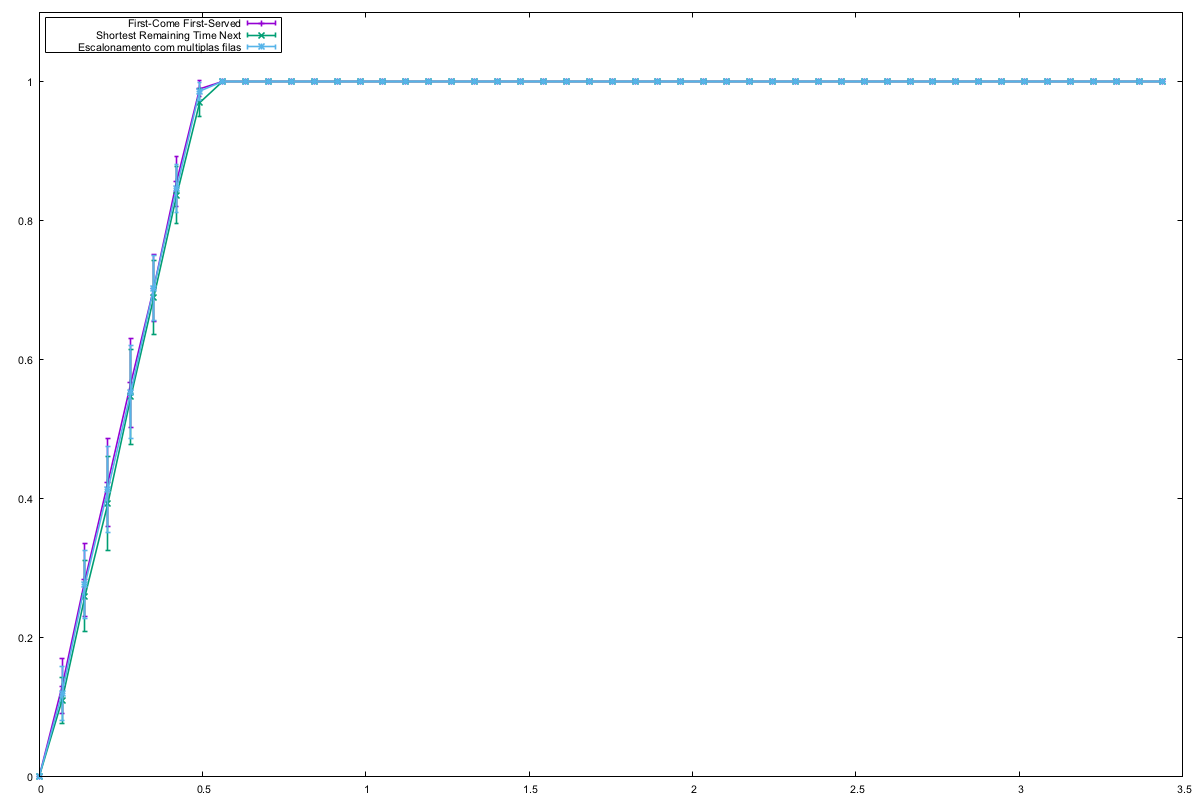
\includegraphics[width=\textwidth]{graphs/testes_capella/result/deadlines-r8-10}
	
	{\tiny No eixo $x$ temos o tempo em segundos que foi adicionado $y$ do processo para determinar o deadline.}
\end{frame}


\begin{frame}{Porcentagem de Deadlines Cumpridos, $n = 100$ e $4$ CPUs}
	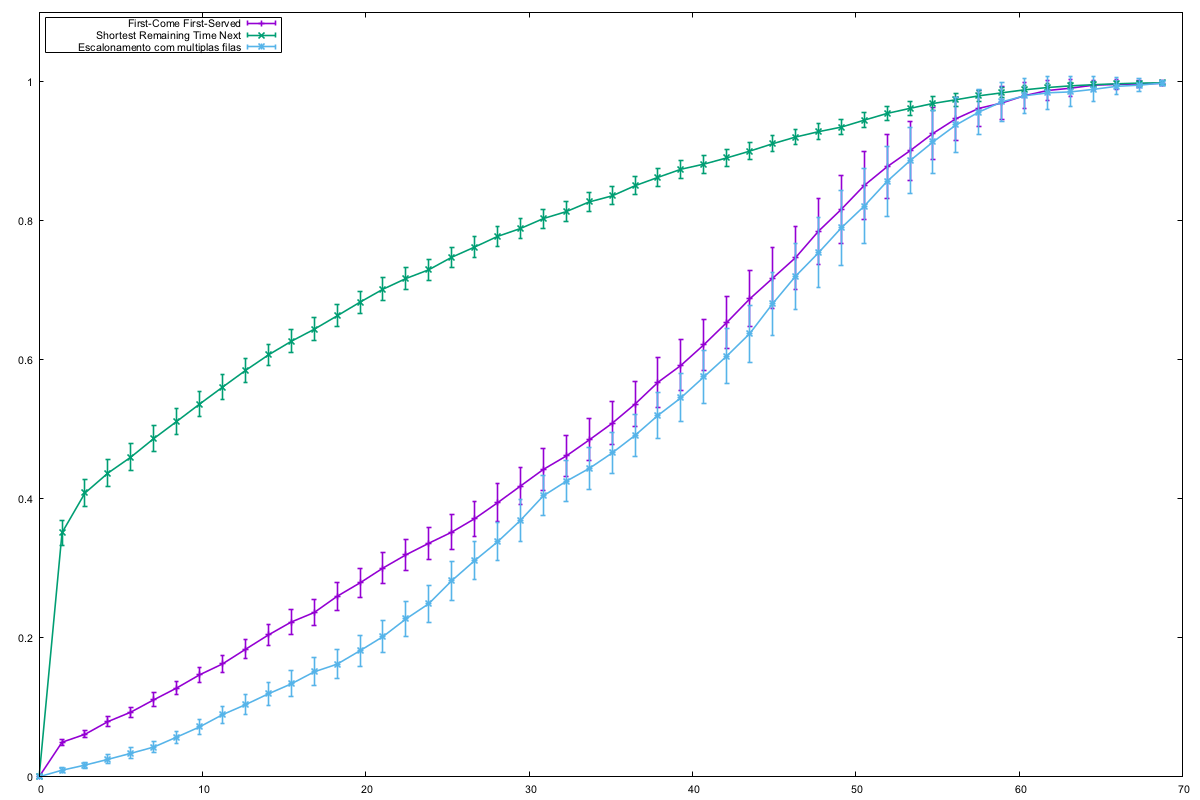
\includegraphics[width=\textwidth]{graphs/testes_capella/result/deadlines-r4-100}
	
	{\tiny No eixo $x$ temos o tempo em segundos que foi adicionado $y$ do processo para determinar o deadline.}
\end{frame}


\begin{frame}{Porcentagem de Deadlines Cumpridos, $n = 100$ e $8$ CPUs}
	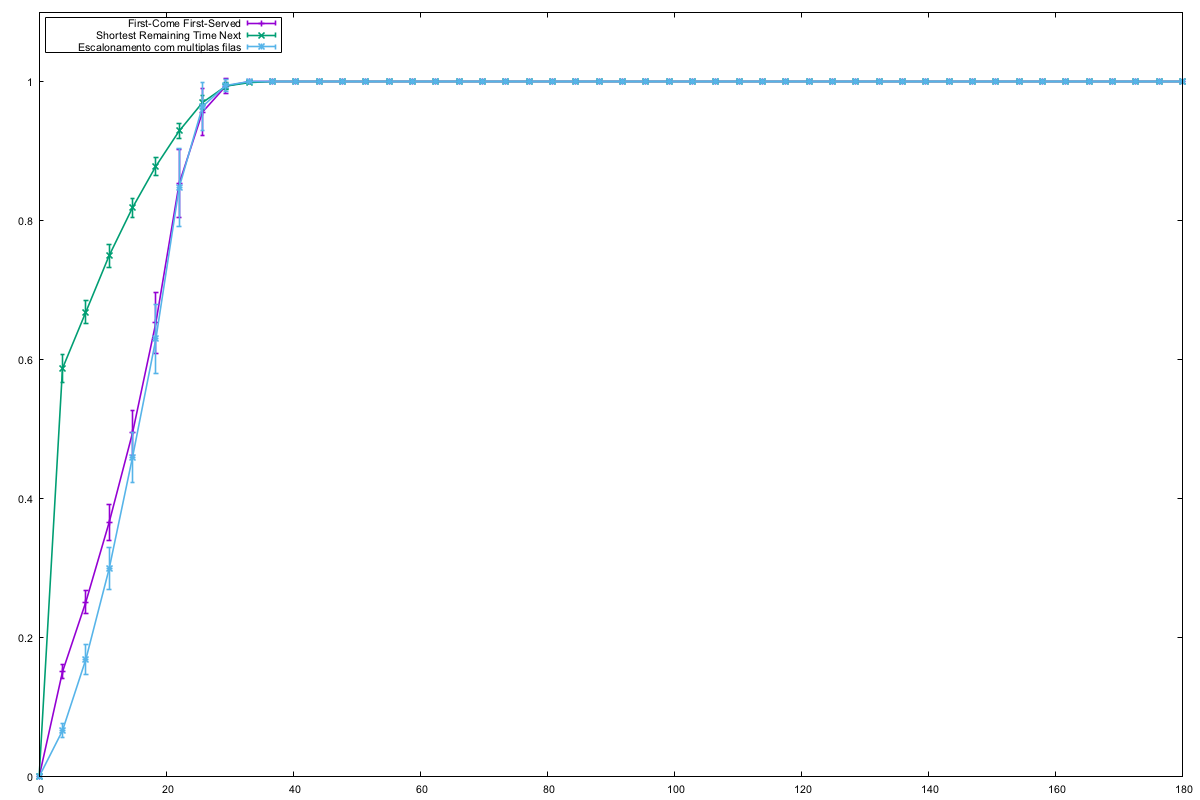
\includegraphics[width=\textwidth]{graphs/testes_capella/result/deadlines-r8-100}
	
	{\tiny No eixo $x$ temos o tempo em segundos que foi adicionado $y$ do processo para determinar o deadline.}
\end{frame}


\begin{frame}{Porcentagem de Deadlines Cumpridos, $n = 500$ e $4$ CPUs}
	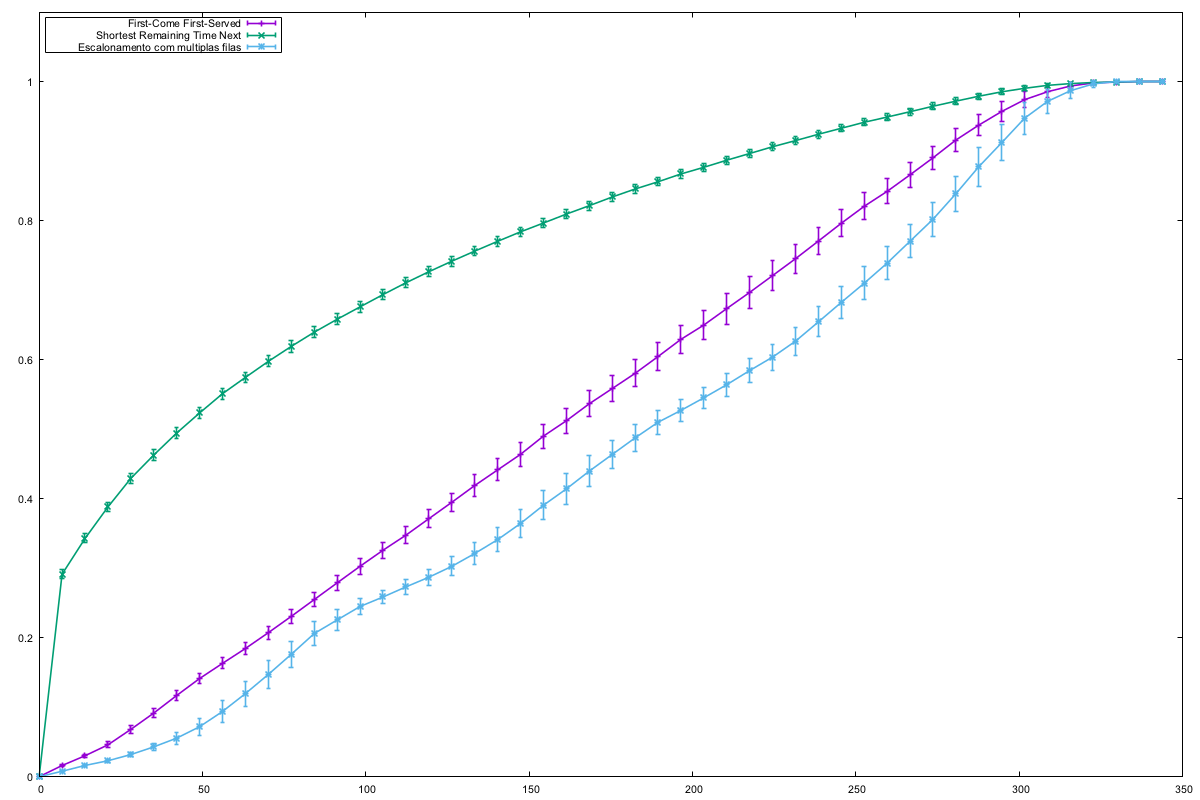
\includegraphics[width=\textwidth]{graphs/testes_capella/result/deadlines-r4-500}
	
	{\tiny No eixo $x$ temos o tempo em segundos que foi adicionado $y$ do processo para determinar o deadline.}
\end{frame}


\begin{frame}{Porcentagem de Deadlines Cumpridos, $n = 500$ e $8$ CPUs}
	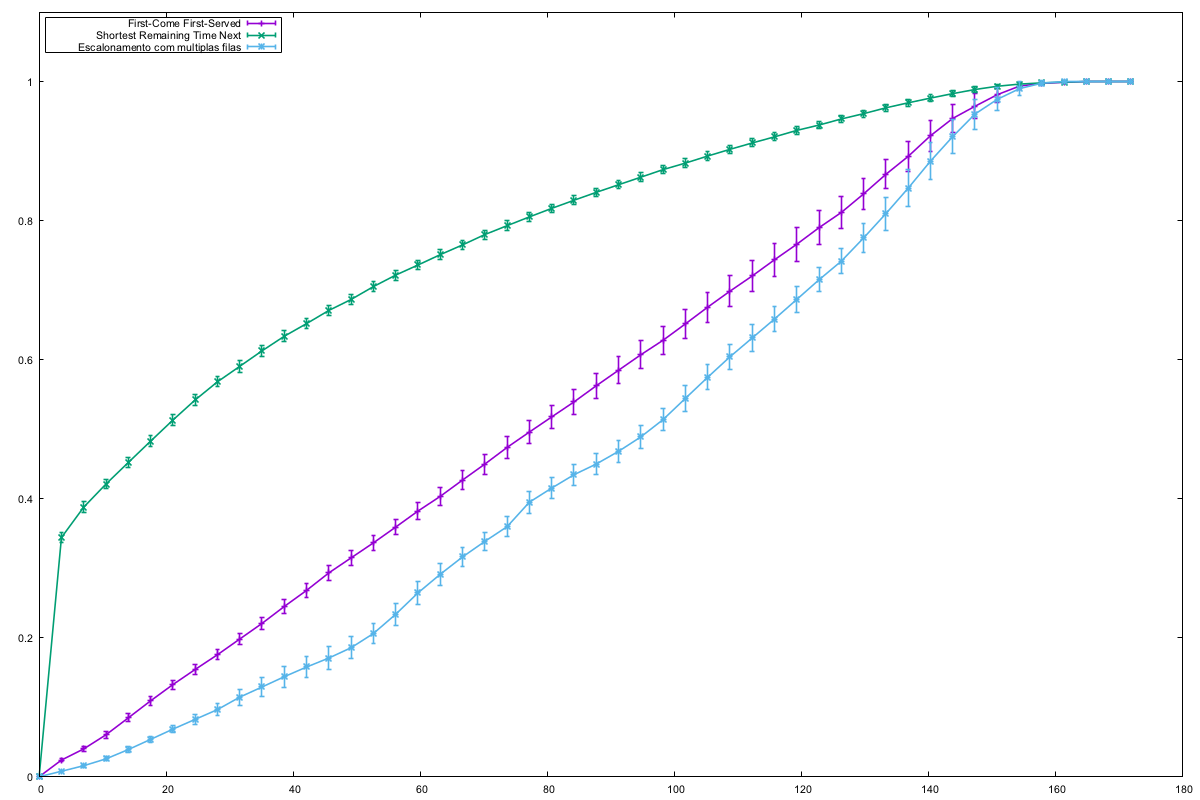
\includegraphics[width=\textwidth]{graphs/testes_capella/result/deadlines-r8-500}
	
	{\tiny No eixo $x$ temos o tempo em segundos que foi adicionado $y$ do processo para determinar o deadline.}
\end{frame}

\end{document}